
In this chapter, we aim to characterise transcript degradation and read truncation from long-read RNA-seq data. Transcript degradation from the 5' end results in truncated reads and a decrease in coverage with increasing distance from the 3' end for a given isoform. Thus, even though the observed degradation occurs from the 5' end, it is helpful to characterise degradation as the resultant decrease in coverage from the 3' end. We formalize the notion of degradation by defining the \textit{degradation rate}. 
\begin{definition}[Normalized coverage]
Let the maximum coverage over an isoform be $\mathrm{cov}_{\mathrm{max}}$ and the coverage at base $b$ be $\mathrm{cov}_b$. The normalized coverage of the isoform at base $b$ is defined as 
\begin{equation}
    \mathrm{ncov}_b=\frac{\mathrm{cov}_b}{\mathrm{cov}_{\mathrm{max}}}
\end{equation}
\end{definition}
\begin{definition}[Degradation rate]
Let $\mathrm{ncov}$ be the normalized coverage over an isoform, and $x$ be the distance in kb from the 3' end. The degradation rate of an isoform is defined as the rate of change in normalized coverage with respect to distance in kb from the 3' end of the isoform:
\begin{equation}
    d=\lim_{\Delta x\rightarrow 0} \frac{\Delta \mathrm{ncov}}{\Delta x}
\end{equation}
The degradation rate of an isoform at a base $b$ with distance $x_b$ away from the 3' end is the value of this limit evaluated at $x=x_b$. 
\end{definition}
Intuitively, the degradation rate can be interpreted as the gradient of the plot of normalized coverage against distance from the 3' end. To illustrate this, we visualise the normalized coverage plots for a hypothetical isoform of length 2 kb with different degradation rates (Fig. \ref{fig:sec-2-hypo}).  
\begin{figure}[H]
    \centering
    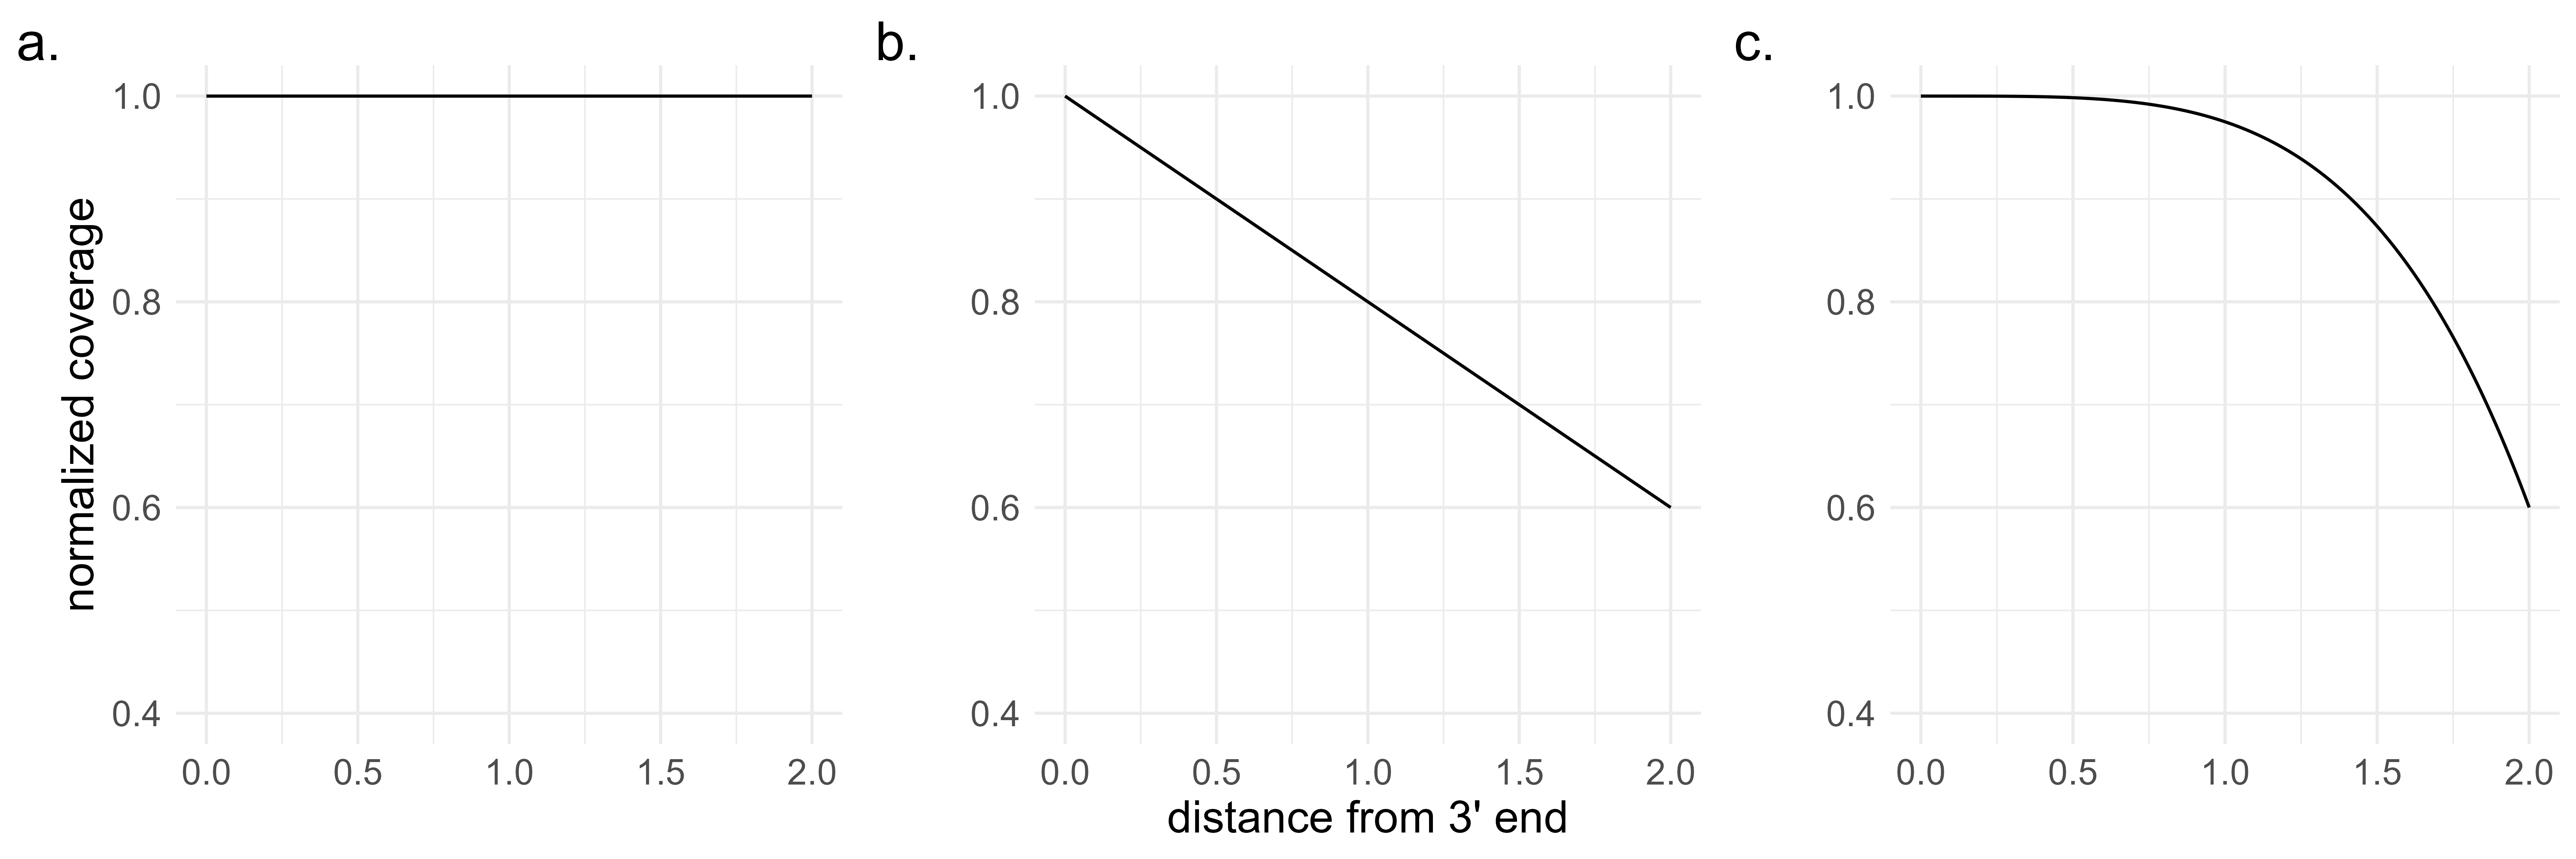
\includegraphics[width=\textwidth]{figures/sec-2-hypo.png}
    \caption[Normalized coverage plots for a hypothetical isoform]{Normalized coverage plots for a hypothetical isoform of length 2 kb illustrating different degradation rates. \textbf{a.} Degradation rate is 0. \textbf{b.} Degradation rate is constant (0.2). \textbf{c.} Degradation rate is variable.}
    \label{fig:sec-2-hypo}
\end{figure}
In Fig. \ref{fig:sec-2-hypo}a, the degradation rate is 0, implying that all reads from the isoform are full-length, and there is no drop in coverage over the isoform body. Conversely, in Fig. \ref{fig:sec-2-hypo}b, the degradation rate (gradient) is a constant value of 0.2 over the isofrom body, implying that for every 1 kb from the 3' end, normalized coverage drops by 0.2. The last plot in Fig. \ref{fig:sec-2-hypo}c shows variable degradation over the isoform body. In particular, the degradation rate is low towards the 3' end and increases with distance from the 3' end.  

In the following sections, we describe our approach for estimating the degradation rate and present findings based on ONT long-read RNA-seq data from common cancer cell lines (A549, Hct116, HepG2, MCF7 and K562) and a human embryonic stem cell line (H9) sequenced as part of the SG-NEx project . 

\section{Degradation rate estimation}

We first sought to determine if patterns of degradation were consistent across transcript isoforms for a given direct RNA-seq dataset. To that end, we selected single-isoform, multi-exon genes from the GRCh38 reference annotations, and further restricted the set of isoforms to those that do not intersect with any other annotated features in reference annotations. These filters reduce ambiguity in the isoform of origin of the reads we use to estimate bias; such approaches were also adopted in \cite{Roberts2011} and \cite{Love2016} for bias estimation in short-read data. Filtering yielded approximately 5,000 isoforms for bias estimation.   

\subsection{Degradation by transcript features}

\subsection{Degradation in spike-ins}


